\documentclass{arsubmit}

\title{Writing Manuscripts with LaTeX2e}
\author{First Author, \and Second Author \and and Third Author}
\date{\small \it{Affiliation, Address, and E-mail}}
\begin{document}
\maketitle
\begin{abstract}
Advanced Robotics is the international journal of the Robotics Society
of Japan.
This is an example file for those who are considering
to write their manuscripts in LaTeX2e and to submit to Advance Robotics.
Approximately 200-word (100-word for short papers) abstract must be 
printed on the first page, followed by the list of keywords (see below).  
The abstract may consist of, for example, the background and the 
aim of the study, the authors' approach, what authors have achieved, 
its evaluations,  and conclusions.  
The original or innovative point of the paper
should be clearly described.
\end{abstract}
{\it keywords}: robot, automaton, mechanical man, android, humanoid

\section{INTRODUCTION}
\label{sec:introduction}

This document illustrates how to prepare your manuscript to submit
to Advanced Robotics in LaTeX format.

What this document says may sometimes conflict with those in our web 
page.  In such cases, follow not this example, but the rules and 
guidelines in the web page.
The aim of this document is just to provide an example file which
can be compiled with our style files.

\section{LANGUAGE}
\label{sec:Language}

Manuscripts must be written in English.  
The editorial board of Advanced
Robotics recommends every author to have the manuscript checked by
professional proof readers because of the following reason:
you should understand
that manuscripts in poor English are sometimes handicapped in the
review processes, and even when the manuscript is acceptable, 
it often takes longer time to be reviewed.

\section{CATEGORIES}
\label{sec:Categories}
A full paper is a paper which describes author's original contribution
%to the robotics.  
to robotics.  
A survey paper is either a review or a tutorial.
A short paper is a paper which describes a result, a particular technique,
or an experiment of general interest.

Full and survey papers should not exceed 6000 words, while short papers
are limited to 4000 words.
\section{FORMAT and STYLE}
\label{sec:Format and Style}

Manuscripts must be typed single-sided on A4 (or US letter sized) papers.

As for the style, please understand our policy that the style file for
the submission should be different from the one for the 
publication.
\begin{itemize}
\item {\bf Manuscript Style}
  \begin{itemize}
  \item It must be as simple as possible for the sake of authors'
convenience.
  \item It must have enough line spacing pitch for the convenience
  of proof read.
  \end{itemize}
\item {\bf Journal Style}
  \begin{itemize}
  \item It must have enough capability to yield beautiful and 
impressive page layouts.
  \item It may demand professional typesetting skills of the user and
    special font sets installed in the compiling system.
  \end{itemize}
\end{itemize}

When you submit your paper, use 'arsubmit.sty' and 'arsubmit.cls,'
which are distributed with this sample file 'sample2e.tex.'
'Arsubmit' document class is almost same as standard 'article' 
document class for
LaTeX2e, except for the 1.5-line spacing, and bigger text area.
In 'arsubmit' class, the well-known macros and environments of
standard 'article' class can be used in the exactly same manner.

As for the journal page image, you can have a good guess by using
'article' class of LaTeX2e, but do not spend your time on solving
minor layout problems.  When your paper is accepted, professional 
typesetters will take care of it to render in beautiful pages.

\section{REFERENCES, EQUATIONS, FIGURES, and TABLES}
\label{sec:References, Equations, Figures, and Tables}
\subsection{References}
\label{sec:References}
References should be listed at the end of the paper in the reference
section in the cited order with consecutive numbers in this way
for books~\cite{AmariNagaoka}, edited books~\cite{PDP}, 
journal papers~\cite{Amari}, and for proceedings 
papers~\cite{IROS}.

\subsection{Equations}
\label{sec:Equations}
Equations and formulae must be typed and consecutively numbered 
%by Arabic numerals in parentheses:
using Arabic numerals in parentheses:
\begin{equation}
  \label{eq:quaternion}
  \omega = 2\frac{dq}{dt}\bar q = 2 \left (
  \begin{array}[c]{c}
-\frac{dq_0}{dt}q_1 +\frac{dq_1}{dt}q_0 -\frac{dq_2}{dt}q_3 +\frac{dq_3}{dt}q_2\\
-\frac{dq_0}{dt}q_2 +\frac{dq_1}{dt}q_3 +\frac{dq_2}{dt}q_0 -\frac{dq_3}{dt}q_1\\
-\frac{dq_0}{dt}q_3 -\frac{dq_1}{dt}q_2 +\frac{dq_2}{dt}q_1 +\frac{dq_3}{dt}q_0
  \end{array}\right ).
\end{equation}

\subsection{Figures}
Figures must be numbered consecutively, and captioned appropriately.
%Photos are also  dealt as figures.
Photos are to be dealt with in the same way as figures.
\label{sec:Figures}
\begin{figure}[htbp]
  \begin{center}
    %\includegraphics{graphics.eps}
    \resizebox{100mm}{!}{\includegraphics{graphics.eps}}
    \caption{Responses of integrate-and-fire type units.}
    \label{fig:evolution}
  \end{center}
\end{figure}

\subsection{Tables}
Tables also must be numbered consecutively, and captioned appropriately.
\label{sec:Tables}
  \begin{table}[htbp]
    \begin{center}
    \caption{Categories of papers and size limits.}
    \begin{tabular}{ccc}
      \hline\hline\\
    Category & 
    \begin{tabular}[h]{c}
    Limit\\
    (words)      
    \end{tabular}
   & 
    \begin{tabular}[h]{c}
    Abstract\\
    (words) 
    \end{tabular}\\
      \hline
    full paper& 6000 & 200\\
    survey paper& 6000 & 200\\
    short paper& 4000 & 100\\
        \hline
      \end{tabular}
      
    \end{center}
  \end{table}

\section{SUBMITTING YOUR MANUSCRIPT}
\label{sec:Submitting your manuscript}

\subsection{Preparing the manuscript}
\label{sec:Preparing_mannuscript}
A manuscript must contain the following materials. All the texts and
information must be written in English, and be typed 1.5-2 line
spacing, single-sided, on A4 (or US letter sized) papers. Available
file type for electronic submission is PDF format only. Total file
size must be less than 3 MByte.

Our 'arsubmit' style for LaTeX2e generates a page which is suitable
for reviewing and proof reading, but it is quite different from the
image of journal page. If you want to know how many journal pages your
paper would be, use standard 'article' class instead of our class. It
will give you a very good estimate.

\begin{description}
\item[Paper title]
\item[Names of all authors]
\item[Abstract]
200 words for full/survey papers, 100 words for short papers. 
\item [List of keywords]
no more than 5 keywords. 
\item [Text body]
Typed or printed single-sided, 1.5-line spacing on A4 (or US letter sized) 
papers, numbered beginning with the title page.
\item [Figures (including photos) and Tables]
Figures and tables must be numbered consecutively, and captioned appropriately. 
Figures (including photos) must have suitable quality for reproduction.
Photos, figures, and tables may appear in the text body.
\item [References]
References should be listed at the end of the paper in the reference section in the order they are cited in the text body. 
\end{description}

\subsubsection*{Note}
\label{sec:Note2}
The principal author is responsible to secure requisite permission from 
his/her employer, and all papers submitted are understood to have 
received due clearance(s) for publication.

\subsection{Submission}
\label{sec:Submission}

Submit your manuscript with author's information from 
``Author's Information Page''.
Advanced Robotics encourages submission of manuscripts in PDF format.
Be sure that the maximum PDF file size does not exceed 3 MB.

\begin{center}
http://www.rsj.or.jp/AR/SendAuthorsInfo.html
\end{center}

\section{CONCLUSIONS}
\label{sec:Conclusions}

A sample \LaTeX2e file for 'arsubmit' document class is provided.
Authors are recommended to follow instructions and guidelines on our web
page if there are any conflicting points with the contents of this document.

\begin{thebibliography}{99}
\bibitem{AmariNagaoka}S. Amari and H. Nagaoka, {\em Methods of Information Geometry},
Oxford University Press (1993).
\bibitem{PDP}M. I. Jordan, An Introduction to Linear Algebra in Parallel 
Distributed Processing, in {\em Parallel Distributed Processing}, 
 D. E. Rumelhart et al. (Eds.), pp.365-422, MIT Press, Cambridge, MA (1986)
\bibitem{Amari}S. Amari, Differential geometry of curved exponential families 
-- curvature and information loss. {\em Ann. Stat.}, 
{\bf 16}, 357-385 (1982).
\bibitem{IROS} R. Hashimoto, T. Masuda, S. Gardella, and M. Wada, 
Solving Optimal Control Problems with Neural Network Learning, in {\em Proc. 
International Workshop on Intelligent Robots and Systems}, Osaka, pp.1127-1132 
(1991)
\end{thebibliography}
\appendix
\section*{APPENDIX}  % This is needed to generate the title 'Appendix.'

\section{AFTER SUBMISSION}
\label{sec:After Submission}

Except for troublesome and very unlucky cases, the review process will be
completed within 20 weeks after the materials arrive at the
secretariat of Advanced Robotics.

If your paper is accepted, the Editor-in-Chief will send you the
acceptance letter.  Then you will be requested to send
biographical sketches and portraits of all the authors.  
We recommend you to
send also the electronic files (floppy disk or CD-ROM in Windows format)
containing your manuscript with them.  It will help shortening the 
typesetting process, and also reduce the number of typographical errors.
Then the secretariat
will forward all the materials to our partner publisher (Brill/VSP).
The manufacturing editor there will help you to refine the English
and to correct errors before your paper is typeset.

By the way, the reviewers are requested to judge without questioning
the authors.  As a result, papers are often judged to be 'Reject but 
Recommend Re-submission'.  Do not be discouraged, it is not a bad news.
Just read what
reviewers advise, revise the manuscript and submit it again.


\section{PUBLICATION CHARGE}
\label{sec:publication charge}

There is no charge for publication except in the case that your paper
exceeds the page limit.

\section{SUBSCRIPTION}
\label{sec:Subscription}

The members of Robotics Society of Japan get benefit of special discount
rate when taking out a subscription to Advanced Robotics.  
Check our web site for detailed information.

\end{document}
